Il a été nécessaire de créer des classes métiers représentant fidèlement le comportement réel des tables contenues dans n'importe quel \sgbd

\begin{figure}[H]
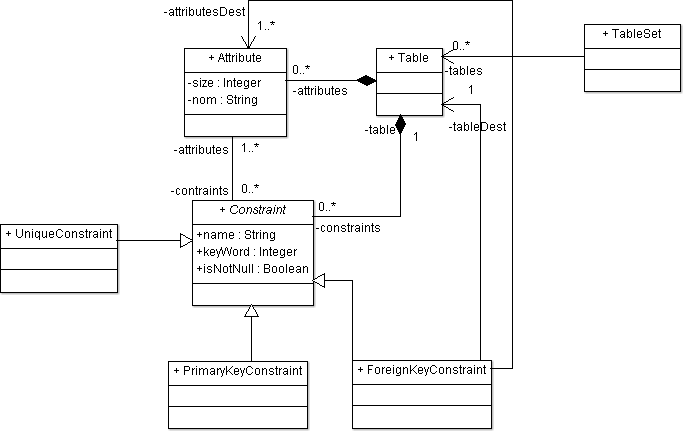
\includegraphics[width=15cm]{images/metier.png}
\caption{Diagramme de classes métiers}
\label{classes_metiers}
\end{figure}


Ces classes ont une particularité, elles peuvent générer du code SQL à partir de leurs attributs ou de différents arguments.
Lorsqu'une table est supprimée, tous les attributs de la table sont détruits et toutes les contraintes composant ces attributs sont détruites également.
Si un seul attribut est détruit, toutes les contraintes qui le compose sont détruites, ainsi, une contrainte \textbf{ForeignKeyConstraint} sera détruite même si elle concerne un second attribut.
\exemple{Une \textbf{fk1} est composé de \textbf{att1} et \textbf{att2} pointant sur \textbf{pk1} et \textbf{pk2} respectivement.
\newline Si l'on supprime \textbf{att1}, alors la clé étrangère ne peut plus respecter la norme et la contrainte \textbf{fk1} sera détruite.}
